\chapter{Návrh krabičky zařízení}

Stejně jako bylo třeba navrhnout veškerou elektroniku, je zapotřebí vytvořit krabičku pro tuto elektroniku. Do ní je zapotřebí umístit hlavní desku řídící elektroniky s~nasazenou senzorovou deskou pro měření osvětlení, baterii a~senzor prachových částic. Krabička byla navržena v~programu SOLIDWORKS a~je koncipována pro tisk na 3D tiskárně. Nejvhodnějším materiálem pro umístění krabičky ve venkovním prostředí je ASA275 a~to díky své odolnosti proti UV zářením a~velkému rozsahu teplot.

Krabička je rozdělena na dvě části, kde v~hlavní části je umístěna veškerá elektronika a~poté kryt, který je k~této hlavní části přišroubován. V~krytu nejsou modelovány závity, ale jsou využity mosazné závitové vložky, které se po vytisknutí zahřáté vtlačí do výtisku. Toto řešení má výhodu ve snadné rozebíratelnosti a~také je pevnější než přímé zašroubování do plastu. Stejným způsobem je přišroubována také hlavní deska. Pro připevnění senzoru prachových částic a~baterie je využito možností 3D tisku a~jsou tedy drženy pouze vložením do předem vymodelovaných pozic a~poté přidrženy krytem celé krabičky. Navržená krabička je vidět na obrázku \ref{fig_Case}. Celkové rozměry jsou $92,4 \times 154,8 \times 39,4$\SI{}{\milli\metre}.

\begin{figure}[h]
    \centering
    \subfloat[][Krabička na elektroniku]{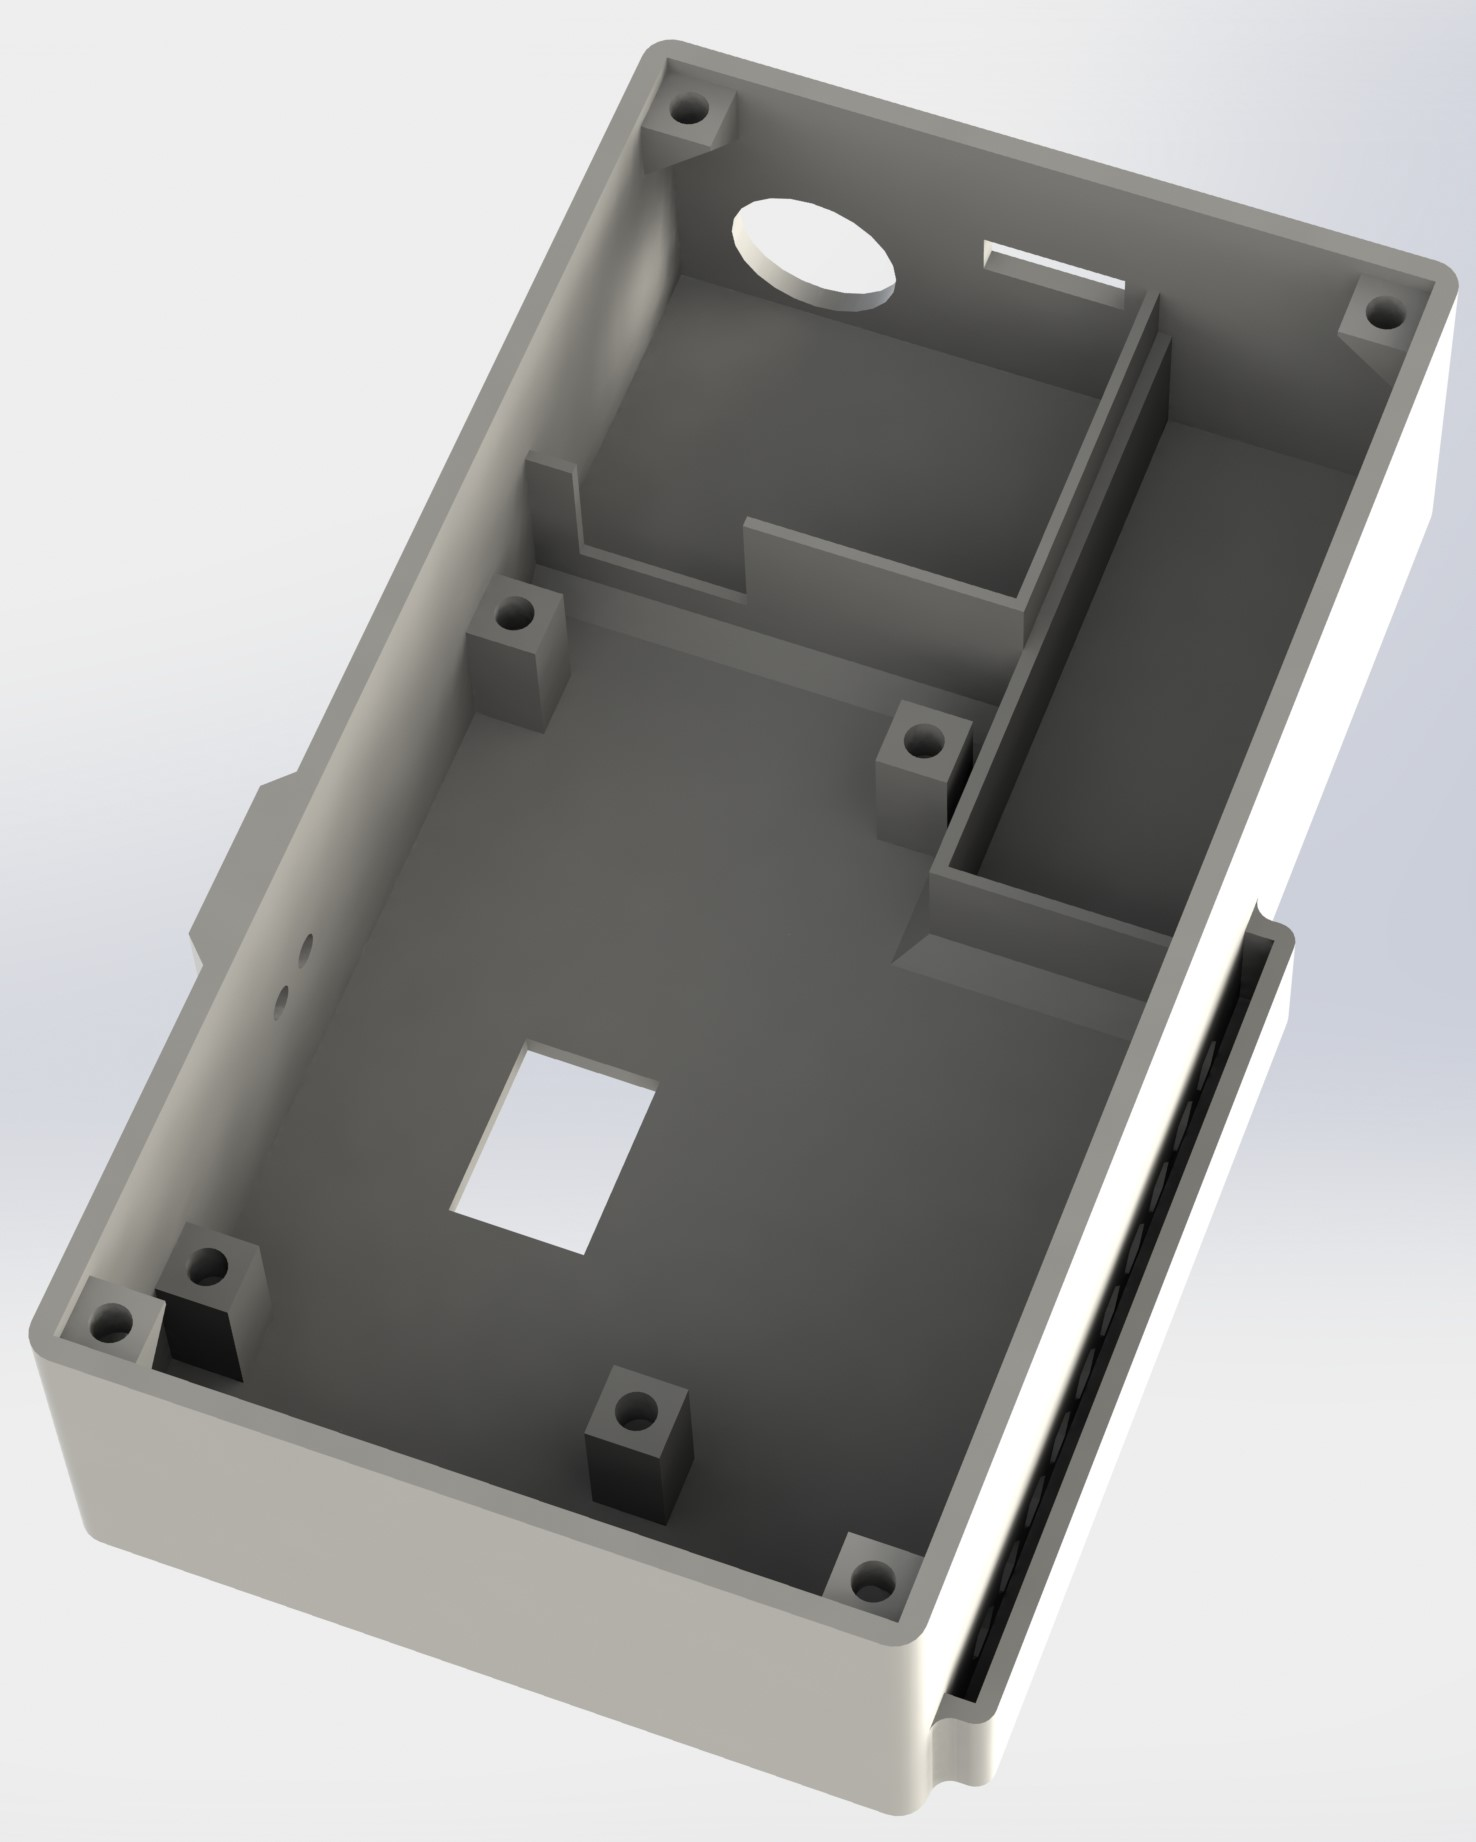
\includegraphics[width=0.55\textwidth]{obrazky/case_bot.JPG}}
    \quad
    \subfloat[][Kryt krabičky]{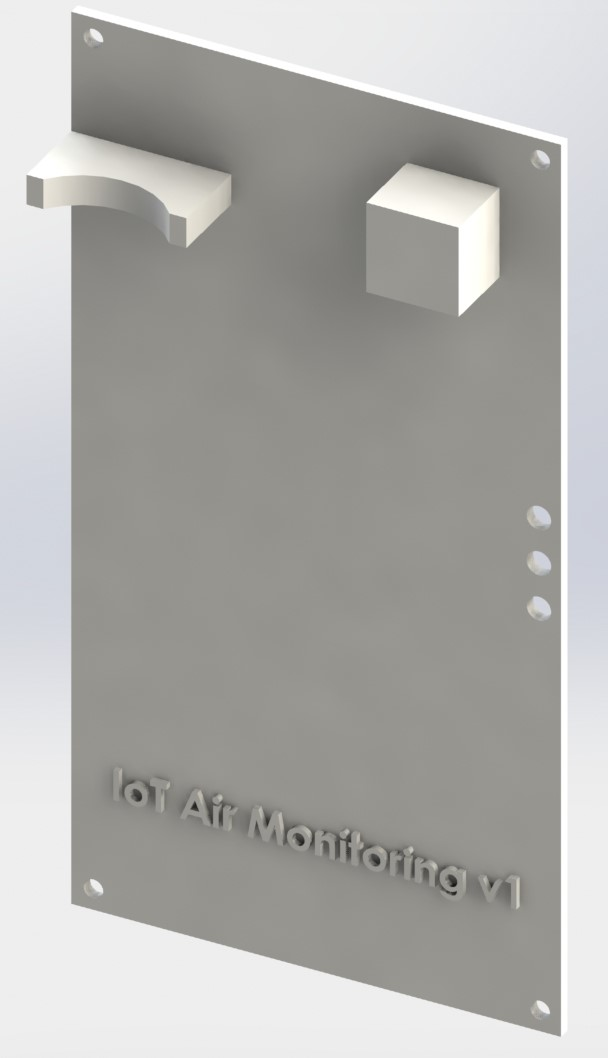
\includegraphics[width=0.39\textwidth]{obrazky/case_top.JPG}}
    \caption{3D model krabičky pro elektroniku.}
    \label{fig_Case}
\end{figure}